%----- Author : Kang Yen -----%
%----- Version: 1.0        -----%
%----- Date   : 2019.06    -----%

\documentclass[12pt]{ksthesis}
\usepackage[cmex10]{amsmath}
\usepackage{amsthm}
\usepackage{latexsym}
\usepackage{./class/psfig}
\usepackage{./class/fancyheadings}
\usepackage{./class/citesort}
\usepackage{graphicx}
\usepackage{subfigure}
\usepackage{amssymb}
\usepackage{algorithm}
\usepackage{algorithmic}
\usepackage{multirow}
\usepackage{cite}

\newtheorem{thm}{Theorem}
\newtheorem{lemma}{Lemma}
\newtheorem{defi}{Definition}
\newtheorem{proposition}{Proposition}
\newtheorem{cor}{Corollary}

\paperwidth=21cm \paperheight=29.7cm

\doublespace

\title{National Cheng Kung University
     \\Institute of Computer and Communication Engineering
     \\Master Thesis}
\author{}

\phdthesis

\Thesisspace

\begin{document}

\begin{preliminary}
%---------- Preliminary ----------%
\setcounter{page}{2} \large


\begin{abstract}
%------------------------- Abstract -------------------------%
\begin{center}

{\Large Implementation of Vehicle Dispatching and Monitoring in a Self-Driving Delivery Emulation System for Urban Areas\vspace{0.4cm}}

\end{center}

\begin{center}

{\large Kang Yen\vspace{0.2cm} \\ Institute of Computer and
Communication Engineering \vspace{0.2cm}\\ National Cheng Kung
University \\ }

\end{center}

\Thesisspace {\large 
Freight transportation plays an important role in daily life. As the e-commence and traffic technology developed, customers have high expectations for the more rapid and more flexible parcel delivery service. However, due to rising labor costs, the delivery mode of autonomous cars is one of alternatives. By reviewing the self-driving technology, the maturity of technology and profitable business model are the concerns. Moreover, so far there is no complete self-driving delivery system in Asia.
 
As a result, the paper integrated traffic simulation software SUMO and mobile application to simulate the package delivery service. Moreover, this study proposed a vehicle dispatching and monitoring system, which can cope with delivery orders, arrange routes, monitor vehicle’s movements, and demonstrate loading and unloading details of trucks. At the same time, this paper proposed dynamic dispatching mechanism consisting of box filtering stage and simple time scheduling stage. The mechanism can judge whether the delivery order could be established. Finally, the paper ran the parcel delivery simulation in the downtown area of Tainan, which showed clear visualization of logistic condition in the simulation results.

Using this proposed system has three advantages. One is that the user can experience more immediate and more flexible delivery service. Second is that administrator can monitor the vehicle’s route and the vehicle’s real-time behavior. Third is that the developer can extend more complex routing algorithm, and add new application on the simulation platform.
}

\emph{\textbf{Keywords}}---self-driving delivery, traffic simulation, dynamic dispatching mechanism, package delivery service.

\end{abstract}

\begin{acknowledgements}
%------------------------- Acknowledgement -------------------------%
\Thesisspace {\large First of all, I would like to express my gratitude to my advisor, Professor Kuo-Feng Ssu, for his valuable advices in my research and encouragement during my time at National Cheng Kung University. I am exceptionally thankful for his endless effort to provide guidance of paper reading and thesis writing.

Besides, I am really grateful to Professors Hewijin Christine Jiau for not only her contributions to the research but also serving on my dissertation committee.
I am obliged to the members of Dependable Computing Laboratory, including Yu-Jung Change, Che-Ming Lee, Wei-Lun Hung, Wen-Chin Lai, and Chun-Ting Po. They helped me a lot and gave me many opinions in my research.
Finally, I would like to thank my family and friends for their support.}

\end{acknowledgements}

\tableofcontents \listoffigures\clearpage

\end{preliminary}
%---------- Preliminary ----------%
\begin{thesis}\large {
%------------------------- Introduction -------------------------%
\chapter{Introduction} \label{Chap:Introduction}

Freight transportation problem is an important issue in our daily lives \cite{Anand2012} . With the development of transportation technology, the customers have the higher expectation on more efficient and more rapid delivery service. Besides, as the self-driving car technology grows \cite{Lutin2013}, the self-driving vehicle delivery begins to be a crucial research topic. After reviewing the self-driving car delivery market, there is no complete self-driving delivery system. 
Before introducing the autonomous cars to the real road network, so far the thesis wants to focus on building the software part of the whole system, which can run package delivery simulation. As the software part of the system can be established, the administrator can get the car’s real-time information including vehicle’s location, the container’s values, and the vehicle’s speed. As a result, in the future the user can apply the above functions into the actual self-driving cars for achieving the goal of system integration directly.

As illustrated in Figure 1.1, this thesis implemented a vehicle dispatching and monitoring system in the red frame. This system includes two main components such as Simulation of Urban Mobility (SUMO) simulator and a SUMO server. The SUMO server was implemented by Traffic Control Interface, which have the access to retrieve the vehicle’s values or manipulate the vehicle’s behaviors on a running road traffic simulation.

\begin{figure}[t!]
\centering
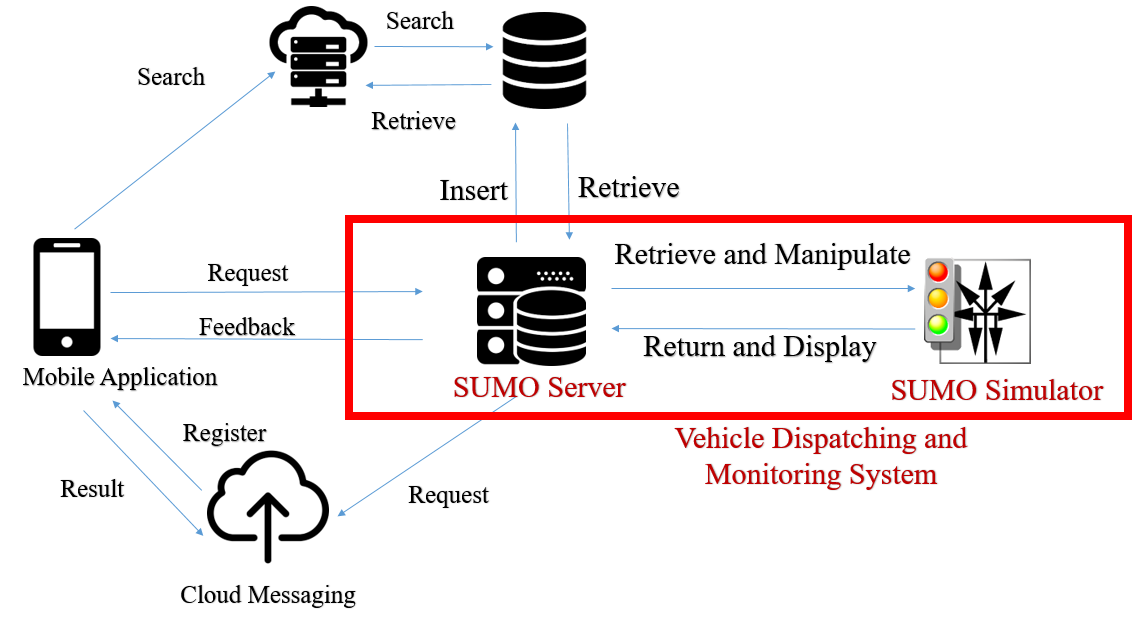
\includegraphics[width=0.85\textwidth]{./Thesis_figures/F1-1_System_Design_Overview.PNG}

\caption{\large A Vehicle dispatching and monitoring system.}
\vspace{0.5cm}
\label{Fig:System_Overview}
\end{figure}

In the previous scheme \cite{Jiang2018}, senders can select their delivery time, but receivers only can wait for the coming parcels passively. This delivery service has the problem that the arrival time of parcels does not match receivers’ available time, which leads to the loss of taking delivery of goods. Hence, the thesis offers a new delivery service where receivers have the chances to select their expected arrival time of the package, which can improve the delivery loss problem. This thesis illustrates the flow chart of the new delivery process including the sender’s part and the receiver’s part.

Besides, the SUMO server develops a dispatching mechanism to deal with the order requests, and arranges the routes dynamically and immediately. In this mechanism, vehicles have to pass through the two stages. First is box filtering stage, which filters out the vehicle without the available space of the appointed box size, and the other vehicles can enter into the second stage named as simple time scheduling stage. This stage would judge whether the order can be inserted into the original time schedule or nor. Moreover, the thesis would demonstrate that the dispatching mechanism would be applied to the scenario of the sender and the receiver in the different ways.

Finally, the thesis installs the SUMO simulator, cleans up the map of the downtown area of Tainan, sets up the parameters, and ran the simulation with five scenarios of the delivery service.

To sum up, the thesis is organized as follows. Chapter 1 describes the motivation of research and the background of self-driving delivery and the purpose of building the system. Chapter 2 presents the related work. The whole system design overview is proposed in Chapter 3. The implementation of a vehicle dispatching and monitoring system is described in Chapter 4. Chapter 5 shows flow charts of the delivery process.  Chapter 6 illustrates how the dispatching mechanism works. The simulation result is presented in Chapter7. Finally, conclusion and future work are discussed in Chapter 8.


  


\chapter{Related Work} \label{Chap:Related}
%------------------------- Related Works -------------------------%

\section{Home Delivery}
As the e-commence and the technology of logistics has developed for several years, this bought about the general tendency in logistics toward higher delivery frequency, single orders, and smaller freight \cite{Visser2014}.

In the freight transportation industry, logistics models can be divided into several types of logistic channel including post, shelf picking, dedicated warehouse, workspace, and home delivery.

Gevaers et al. developed a cost simulation tool, which showed that the Last Mile delivery is one of the most expensive stages of the entire e-logistics chain \cite{Gevaers2014}. Besides, in the Last Mile delivery, the most widespread delivery mode is home delivery.

As the result, home delivery (HD) is a crucial topic to discuss, retailers delivered a large amount of the daily consignment to the customer’s home. So far home delivery can be a delivery point to one’s home address, to another address, or to a pickup point  \cite{Zhou2016}. 

However, there are some issues about home delivery, including delay of delivery service, the customer’s absence at home, and too long delivery time. Thus, to meet the increasing demand of more rapid parcel delivery service, a small aerial vehicle is proposed by the professors in George Mason University \cite{Ali2015}.

A multi-rotor aerial vehicle can provide the fast and urgent parcel delivery service such as rapid food delivery and remote medical supply delivery. However, this application has some design technical difficulties, which includes extending battery life, handling the increasing weight of the parcel, and dealing with the sudden climate change \cite{Ali2015}. In one word, an aerial vehicle has lower reliability, scalability and capacity than a delivery truck.

Moreover, \cite{Sawadsitang2018} introduced a joint ground and aerial delivery service framework. The framework consists of two delivery modes, which can complement each other due to their unique features and benefits. With this integration of ground-based delivery and drone delivery, the approach not only can cope with sudden service interruption like accident, but also can maximize service quality and minimize cost. However, this approach has the problem of the uncertainty in customer’s demand and computation time of routing the delivery path. 

%% [9], [10]
In some metropolitan areas in the U.S. like Seattle, \cite{Sheth2019} deployed alternative delivery mode such as cargo bikes. Due to the increasing freight volumes on the road and scarce road space, cargo bicycles are being utilized for the last mile deliveries in several urban cities \cite{Melo2017}. The advantage of using delivery bikes is that cargo bicycles are not encumbered by the same parking and congestion constraints as trucks. However, the disadvantage is that cargo bikes are less cost effective for greater distances than delivery trucks.

%% [11]
In China, \cite{Delivery2017} showed that JD.com, which is the largest e-commence platform by revenue, used autonomous driving vehicles to hit the open road in Beijing. The vehicle can store up to thirty containers, and can travel 15 km/hr. The current concerns of this approach are the autonomous driving technology and government regulations.

\section{Traffic Simulation}
SUMO is an open source traffic simulation package including net import and demand modeling components. Besides, SUMO helps to investigate several research topics, which includes route choice and simulating vehicular communication  \cite{Krajzewicz2007}.

%% [13]
\cite{10.1007/978-3-662-45079-6_5} introduced the real-time I/O data interface and proposed an approach to building up a Web service. Beside, by knowing the commands of traffic control interface (TraCI), the user can handle the communication with SUMO Traffic Simulation Suite. Finally, \cite{10.1007/978-3-662-45079-6_5} demonstrated an example of the code, which provides the base for a new Web service called TraaS (TraCI as a service).

%% [14]
\cite{Tunku2016} showed the transportation simulation for food distribution. The author used TraaS to assign trucks backup when the original tricks unable to cover the destination shops at certain time threshold, and re-route the path for the backup vehicles.

%% [15]
\cite{Kendziorra2015} aims to achieve simulation scenarios in which incidents occur, and introduced the implementation of logistic transport. The concept of freight and goods was implemented to enable the simulation of good traffic, which consists of the containers and stop.



\chapter{System Design}\label{Chap:Architecture}
%-------- System Architecture--------%

\section{System Overview}



This thesis designs a self-driving delivery simulation system, as illustrated in Figure 3.1, the system consists of five components, including the mobile application, the TraCI server, the SUMO simulator, the back-end server, and the database. In this system, the mobile application is a platform which can let the user place a delivery order for shipping cargos and track the user’s orders. After a user issues a delivery request on the mobile application, it will be sent to TraCI server. The server will do the dispatching mechanism to assign a truck which meets the conditions to receive the cargo, and it will be displayed on SUMO simulator by TraCI commands. Moreover, the data about order’s information will be uploaded to the database if the assignment is successful, and the user can view the order’s status on the mobile application by connecting to the back-end server. When the truck arrives at the address of shippers or receivers on the simulator, the TraCI server will send a message to the mobile device to notify the user of this event through a cloud messaging service. Moreover, the server will also send a message to notify the receiver that the pickup time of the cargo can be selected already when the truck has arrived at the sender’s address. All the simulated process can be observed on the SUMO simulator. The features of each component will be described in detail in the following sections.

\section{Mobile Application}
In this system, the main object to develop the mobile application is to simulate the real user scenario. The features of the mobile application include registration and login of the user accounts, placing the delivery order, and tracking established orders. The function of each part is depicted as follows.

\subsection{Registration and Login}
When the mobile application is launched for the first time, a token will be generated. If a user sign up and sign in his/her account, the token will be uploaded to the database. The TraCI server can send a notification to the mobile device by this token while the truck arrives at the target. On the other hand, the user-related data like username will be stored in the device’s memory when the user sign in, and it can be used to generate the delivery order and track the user’s orders. The process will be described in the next two segments.

\subsection{Placing the Delivery Order}
In order to simulate the real user scenario, we implement a function that the user can place an delivery order. First, the user needs to fill out the order’s information which includes size, receiver’s username, sender’s address, receiver’s address, and so on. Then, the address will be displayed by google map service so that the user can confirm the correction of location. After that, the user can choose the arrival time of the truck, and send the delivery request to the TraCI server. The request contains user-related data and order’s information, and the server will do the dispatching mechanism by these information and the road condition of the SUMO simulator. The order will be uploaded to the database if the request is accepted. Otherwise, the TraCI server will return a error message to the application to notify the user that there are no trucks can arrive the address at the appointed time.

\subsection{Tracking Established Orders}
After the order is established successfully, the user can track the orders’ status by using the function of tracking orders. In this function, the user can examine the orders which were sent by himself or others. Besides, if the user is a receiver, he can choose the pickup time of the cargo after the truck arrives at the sender’s address. In our view, the receiver should select the pickup time only after loading of the cargo because the system must ensure the cargo is ready to be delivered. In addition, the system provides a function to examine the orders by inputting the order number instead of login. It let the administrator can search all orders of users conveniently on the mobile application.

\section{TraCI Server and SUMO Simulator}
In our system, the TraCI server is response for receiving the user’s requests of delivery, doing the dispatching mechanisms, uploading and updating the order’s information of users, and communicating with the SUMO simulator to get the data of road conditions and dispatch the truck on the simulator. This thesis deals with processing of received data and uploading data of order’s information to the database.
As illustrated in Figure 3.2, after the user places an order with the TraCI server, the order’s data will be stored in a queue of the dispatching requests. The socket program can know the request whether it is sent by a sender or a receiver according to the data, and it will store extra information like the truck number and the container number if the request is sent by a receiver. It is because that the server needs to know which trucks to be dispatched. The server will check the queue continuous, and do the dispatching mechanism if there are any requests in it. If the dispatching is successful, the server would insert or update the order’s information to the database by the database API and send a message to the mobile application through the socket. Otherwise, the server will notify the user that this arrival-time is unavailable by another message. Moreover, the TraCI server will change the dispatching schedule table on the basis of the above result, and it will do the corresponding commands to the SUMO simulator so as to change the selected truck’s route.
After the delivery tasks are assigned to the trucks, they will drive along the designated routes, and the system administrator can observe the trip and the parking place of each truck in the simulator. When a truck arrives at the target, the TraCI server will send a notification to the mobile device through the cloud messaging service to simulate the real situation. Then, after five minutes, the server will simulate the uploading and unloading of the cargo, and it will also notify the receiver that the arrival time can be selected if the target is a sender’s address. All of the above event will change the order’s information, and the server will update it to the database in each time. These changes can be observed on the mobile application by using the feature of tracking orders. Finally, the status of the order will be set to “received” by the server instead of being deleted when the delivery is over. Hence, the records of users’ order can be viewed on the database or the mobile application. The implementation of the cloud messaging service will be described  in Chapter 4.

\section{Back-End Server}
The TraCI server would spend much time doing the dispatching mechanism and simulating the process of transportation, and it will causes the computing delay. To keep the simulation precise, the gap between simulation time and actual time has to be shorten. Hence, we built another server in order to reduce the workload of the TraCI server. In our system, the back-end server is in charge of communicating between the mobile application and the database. It provides a interface by which the user can query or insert data to the database. The works of the back-end server include handling login and registration of user accounts, querying the order's data when the users track their orders, and showing the data of cities, counties and townships when the users are filling in an order form. The mobile application accesses to the database through the TraCI server only if users place a delivery order, so it can reduce the burden of communication on the TraCI server as much as possible. The next section will introduce the design of data formats which are used when the back-end server do the database commands.



\section{Database}
As discussed above, the simulation-related data in our system are stored in the database. The database is composed of four table, they will be described and discussed in this section. 

The first table named user-table keeps the account information of registered users. 
Table 3.1 shows the data format of user-table. As mentioned in chapter 3.2.1, the attribute device\_key is the token generated by the application. The token is assigned to the device rather than the user, and it will be updated when the user logins on different devices. Therefore, the TraCI server can know which device should be notified. The attribute "username" is applied to identify users who place the order, and the others would be used on the future work. 

The second table and the third table are county table and township table. The data format of the two tables is presented in Table 3.2, Table 3.3. The administrative district data of Taiwan are stored in the both tables. These data will be shown on the mobile application when the user wants to select the address of the shipper or receiver; therefore the typo can be reduced so that the process of geocoding can be performed better. The geocoding technology will be mentioned in Chapter 4. Furthermore, it provides scalability, if the range of the simulation becomes larger, the administrator can easily expand regional options by adding data to the database. 

The last table is order table. As shown in Table 3.4, it retains information of the user’s order, and part of them will be explained in this section. The attribute "status" represents the situation of logistics activity, such as "on the way to the receiver’s address". In addition, it is the criteria whether if the receiver can designate the arrival time. The attribute "sender\_name" and "receiver\_name" are used by the TraCI server to determine users which the server will notify. The latitudes and longitudes transformed from senders’ addresses are stored as "sender\_lat" and "sender\_lng", and the same is true for the receivers’ addresses. The attribute "sender\_time" and "receiver\_time" are the arrival time that users select on the mobile application. The TraCI server will exploit these locational and time information to make the dispatching schedule and trip of each truck. Other attributes recorded by order-table may be analyzed in the future work. 
  



\chapter{System Implementation}\label{Chap:System_Implementation}

\section{Mobile Application}


Compared to other mobile operating systems, Android OS holds 86.7\% market share according to the survey. It is the most widely-used operating system in the world. Given that the self-driving delivery will be popularized in all walks of life soon after, Android OS is the most suitable system for developing of the mobile application. The application is built by the Android Software Development Kit (Android SDK), and it is developed on Android Studio which is a Integrated Development Environment for Android. Android Studio provides a preview of the user interface and it has the built-in support of Google Cloud Platform. Consequently, it is a appropriate way to construct the mobile application of the system. Furthermore, Google Map SDK for Android and Google Geocoding API were added to the mobile application, the former enables the application to display the map of simulation and mark the address, the latter is able to transform the street address into latitude and longitude.

In order to send the messages to notify the users that the truck arrived, a cloud solution for messages and notifications is included in the self-driving delivery system. Firebase Cloud Messaging (FCM) is a service provided by Firebase, a subsidiary of Google, and it facilitates messaging between the mobile application and the server built by developers. As illustrated in Figure 4.1, there are three components involving in the process of message passing, including the mobile application, FCM and the server that intends to send notifications (i.e., TraCI server in this thesis). When the mobile application is installed on the mobile device and launched for the first time, it will send a registration request to FCM through FCM SDK. Then, the FCM server will generate a corresponding token for the device, and return it back. The token would be uploaded to the database if users log in. Conversely, when users log out, the token in the database will be removed to prevent the server from notifying the wrong users. According to the tokens stored in the FCM server, the messages sent from the TraCI server will be forwarded to the relevant device by FCM.

The user interface of the mobile application is illustrated in Figure 4.2. As shown in Figure 4.2a, the homepage of the application is constituted by the buttons of the main functions. We developed a simple registration function of user account, which is shown in Figure 4.2b. Before the users log in, the FCM token is stored in the memory of the device. The user can be found on different mobile device by logging in. 

The established order can be viewed on the page of tracking orders shown in Figure 4.2f. The user can slide the tabs which are above the page to switch between orders sent by himself and by others. The detailed information would be displayed while the user click an order, which is shown in Figure 4.2g. If the user is a receiver in an order, he can choose the pick-up time of the cargo according to the status of logistics activity. The page is the same as Figure 4.2e. Besides, if the user or system administrator want to examine the orders of different users, the last function in the application can be utilized. Figure 4.2h exhibits the order searching page, the order can be looked up by entering the order number. There are some features that have not yet been implemented, they are not necessary but can be used to improve user experience or analyze the  user behavior. These will be mentioned in Chapter 5.


\section{SUMO Server and Simulator}

\subsection{Simulation Environment Setup}

The simulation of the delivery process is implemented on SUMO[], “Simulation of Urban Mobility”, which is an open source, highly portable, microscopic and continuous traffic simulation package. The example of roads, vehicles, junctions and other road information are included in the package, and there is the graphical simulator certainly. TraCI is an interface that provides the access to SUMO simulator by using a TCP based client/server architecture. It was implemented in various programming language, such as Python, C++, Java, and so on. In this thesis, TraaS is employed to be the control interface of the simulator. It is a java library for working with TraCI, and it provides plenty of commands to manipulate the simulated objects. For instance, the developer can change the route of a vehicle by certain commands.

The self-driving delivery system is designed to supply a small-scale logistics service in cities. As illustrated in Figure 4.3, the road network environment of simulation is an approximate 50 km2 area, which is a partial region of Tainan, a city of Taiwan. The resource of the map data is gained from OpenStreetMap[], which is a is a collaborative project to create a free editable map of the world. There are 25069 road segments and 6785 junctions in the simulation, and the traffic lights are deployed on the junctions using the real world data. In the beginning of the simulation, three trucks are generated on the roads randomly, and they drive along random routes until the end of the simulation. The maximum speed of trucks are set to 5 m/s according to the average speed estimated by Google Map. The delivery task can be assigned in any time.

\subsection{Build the Socket Server}
For purpose of communicating between the mobile application and the simulator, we built a SUMO server to receive the data transferred from the mobile device and command that the simulator perform delivery task. The SUMO server is composed of a socket server and a main simulated program, which are both developed in Java language. This thesis copes with the socket server part and operations of database API.
When the simulation starts, the socket server will listen to the incoming connections from mobile applications. It is programming with a multi-client architecture, and the demand of users can be completed in a short time. Hence, the system can serve considerable users simultaneously. The user’s request will be stored in the request queue when the user connects to the socket server, and the data format of the request is represented by JSON (JavaScript Object Notation). The simulated program would check the queue in each simulation second. If there is any request, it will be forward to the dispatching mechanism. The order information would be uploaded to the database using JDBC if the dispatching is successful. JDBC (Java DataBase Connectivity) is an API for Java to access the database. The database and the SUMO server are built on the same computer because of the consideration of security, the data can be transferred directly to the local end. The simulation process will display on the GUI of the simulator so that the system administrator can confirm the information of trucks and containers. After the dispatching command is appointed to the truck, it will travel on the new trip. The changes of routes and the parking places can be observed on the GUI, which is shown in Figure 4.4. Moreover, the FCM service is also implemented in the SUMO server, it would send the message to users through the FCM server using the token acquired from the database.

\section{Back-end Sever}
To avoid the leakage of sensitive information of the database, users can not connect to the database directly. Instead, the system take the back-end server as an interface to access to the database. The back-end server is a web server, which is built using Apache HTTP Server. The service which receives query requests from users and operates the database is implemented with PHP program. 
The mobile applications connect to the back-end server by HttpUrlConnection. It is a Android function which make the application communicate with the web server by HTTP protocol. According to the HTTP URL, the web server would execute the PHP program to do the SQL commands of the database. The result returned from the database will be forwarded to the mobile application by the web server. 

\section{Database}
The database of the system is developed with MariaDB 10.1.32. MariaDB is a community-developed, commercially supported fork of the MySQL relational database management system. It inherits the advantages of MySQL. Hence, MariaDB supplies the JDBC driver, and the database API for PHP. This is highly useful for the development of our system. To deal with the administration of the database, phpmyadmin is employed in this thesis, it is a graphical, free and open source tool written in PHP. It allows the developer to manage the database with the use of a web browser. The records of orders can be exported for the subsequent data analysis.
The current goal of the system is to  achieve the urban-wide delivery. Therefore, the information of the administrative districts are stored in county table and township table of the database. There are three City in county table currently, including Tainan City, Taichung City, Taipei City. In the simulation of this thesis, only the map of Tainan City is constructed in the simulator, and the simulated districts involve East District, West Central District, North District, South District, Anping District and Yongkang District. The data are referenced from the Ministry of the Interior’s Open Data (MOI Open Data).







%----------- Simulation --------------%


%------------------------- Simulation -------------------------%

\section{Simulation Setting}

\subsection{Simulator}
SUMO is used to be the simulator for running the parcel delivery simulation [12]. “Simulation of Urban Mobility”, or “SUMO” for short, is an open source, multi-modal traffic, highly portable, microscopic and continuous road traffic simulator. The method to control the SUMO simulator is to use the TraCI client Python Application Program Interface (API), which is available in SUMO packages.

\subsection{Road Network}

The dataset, which was acquired from OpenStreetMap \cite{Haklay2008} , uses the road network of part of Tainan, which is the south of Taiwan. The region of the selected road contains the partial Tainan East District, Tainan West Central District, partial Tainan North District, partial Tainan South District, and partial Tainan Anping District.

The road network, which is pruned by estimating unreachable streets and roads for a truck, contains 25069 roads segments, and 6785 junctions with approximately $50km^{2}$ in the downtown of Tainan.

\begin{figure}[H]
\centering
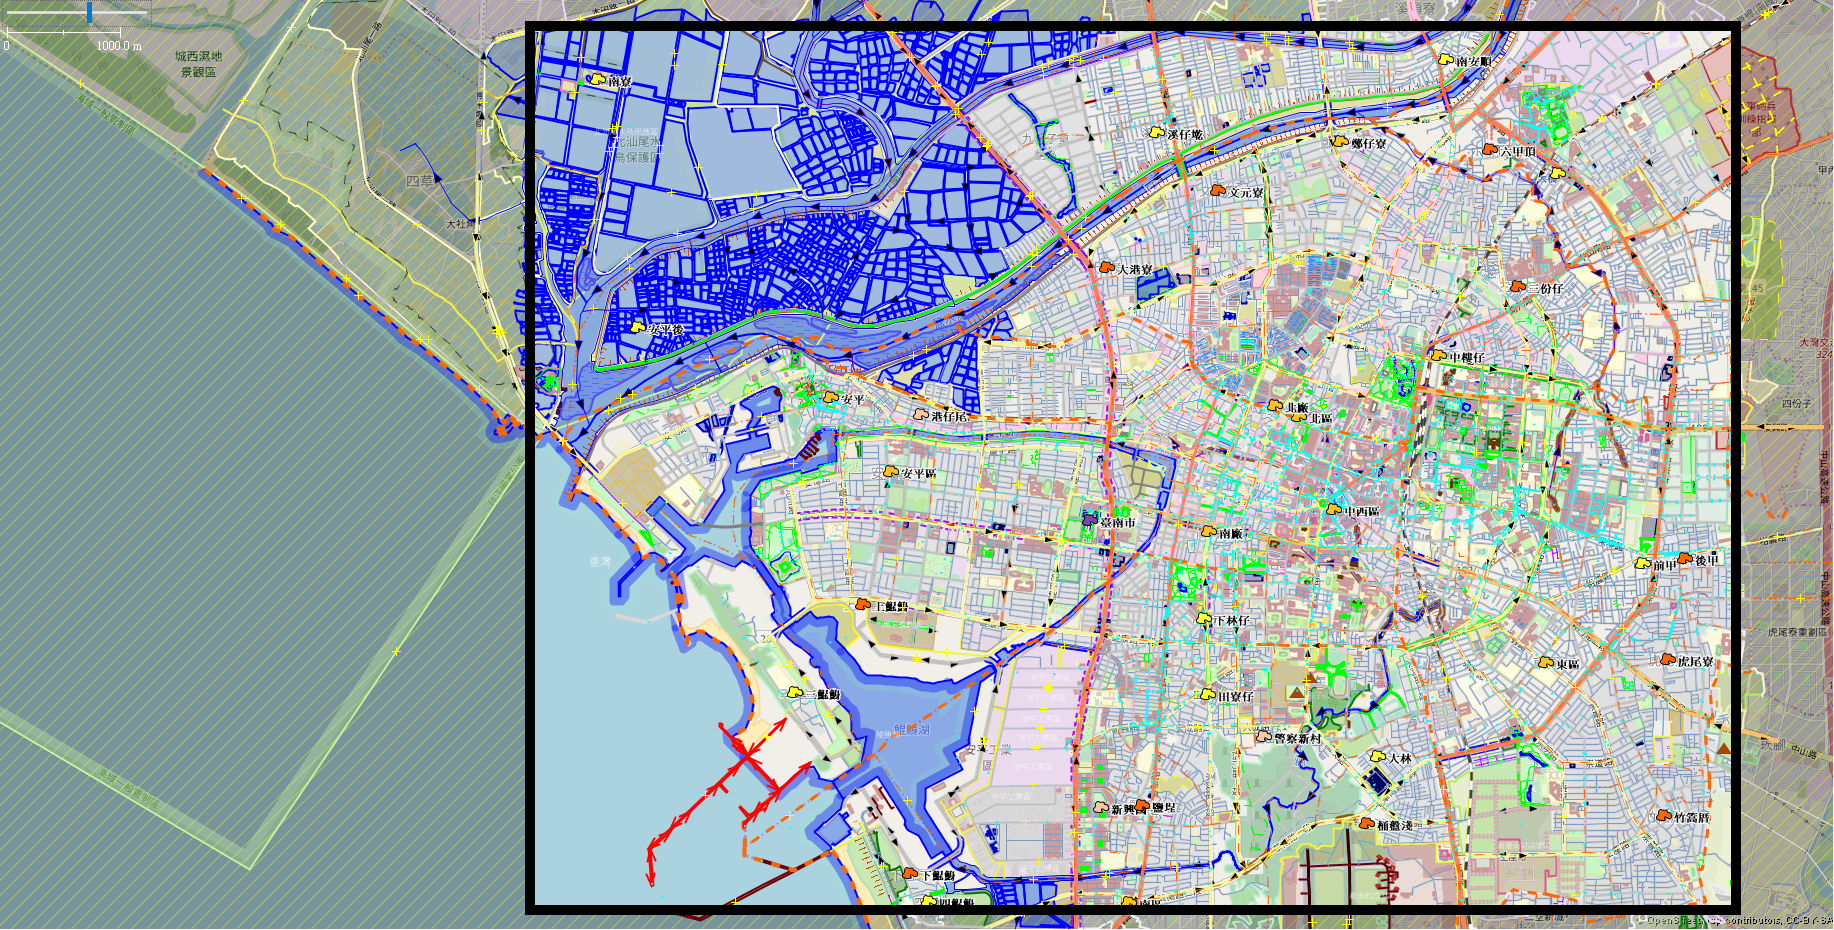
\includegraphics[width=1.0\textwidth]{./Thesis_figures/F7-1_Openstreetmap.PNG}
\caption{\large Downtown area of Tainan in OpenStreetMap.}
\vspace{0.5cm}
\label{Fig:DowntownArea_in_OpenStreetMap.}
\end{figure}


\begin{itemize}
\item
Figure 7.1 shows the road network on OpenStreetMap.

\item
Figure 7.2 illustrates the road network of truck passable segments on SUMO Map.

\item
Figure 7.3 shows the selected road network on Google Map.

\end{itemize}

\begin{figure}[H]
\centering
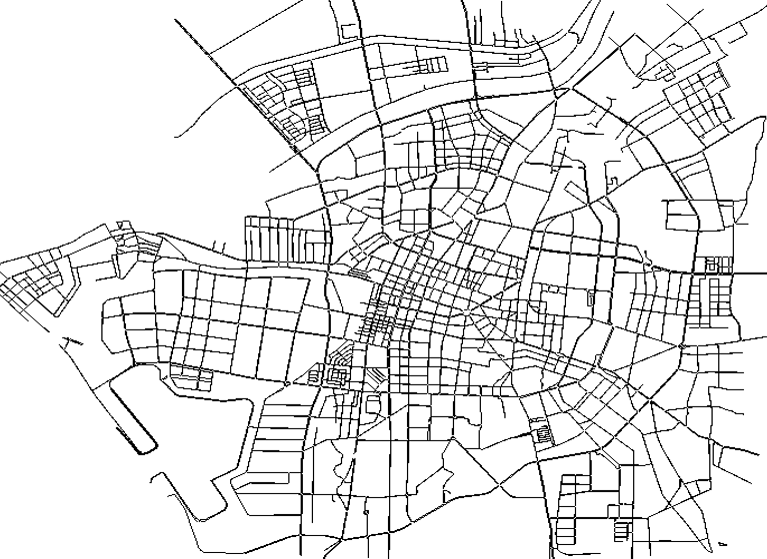
\includegraphics[width=1.0\textwidth]{./Thesis_figures/F7-2_SUMOMap.PNG}
\caption{\large  Service region of the experiment on SUMO.}
\vspace{0.5cm}
\label{Fig:SUMOMap}
\end{figure}

\begin{figure}[H]
\centering
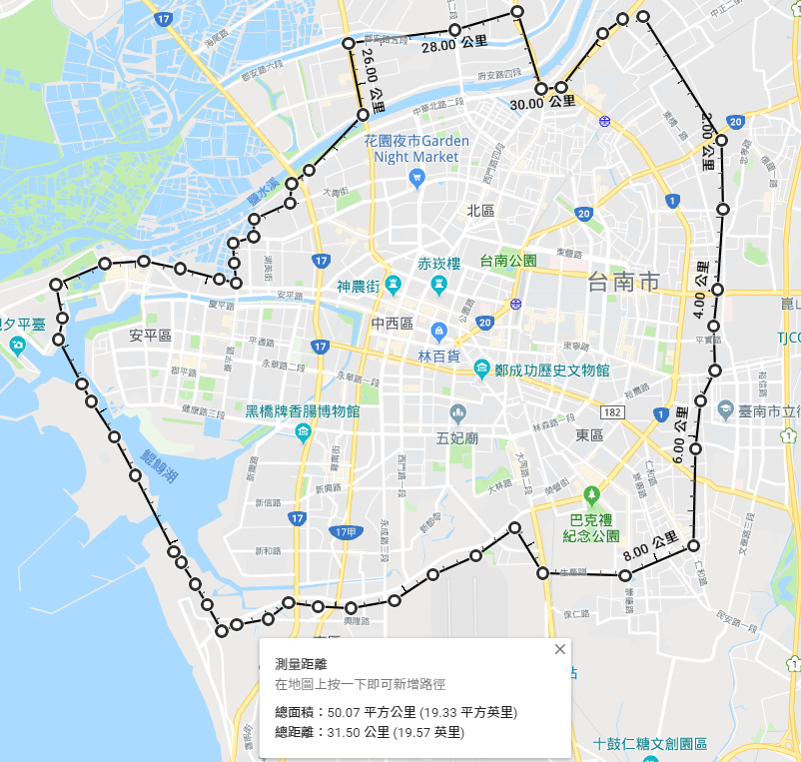
\includegraphics[width=1.0\textwidth]{./Thesis_figures/F7-3_GoogleMap.PNG}
\caption{\large Service region of the experiment on Google Map.}
\vspace{0.5cm}
\label{Fig:GoogleMap}
\end{figure}

\subsection{Parameters}
Parameters of the simulation are showed in Table 7.1. Note that the number of trucks is three from the simulation time $T_{start}$ to $T_{end}$. 
Then, the maximum speed of truck is 18 km/hr, and the range of speed limit on each lane is 10-100 km/hr. It is noteworthy that trucks will not exceed the speed limit on each lane even the truck has a higher maximum speed. Besides, a truck has nine boxes which are grouped by small size, medium size, and large size. The capacity of each box size is three. Then, the loading process time is five minutes, and the unloading process time is five minutes as well. Finally, when the SUMO server counts the travel time of the vehicle, which is equal to the driving distance divided by the estimated average vehicle speed. Thus, the estimated average vehicle speed is 14.4 km/hr.

\begin{figure}[H]
\centering
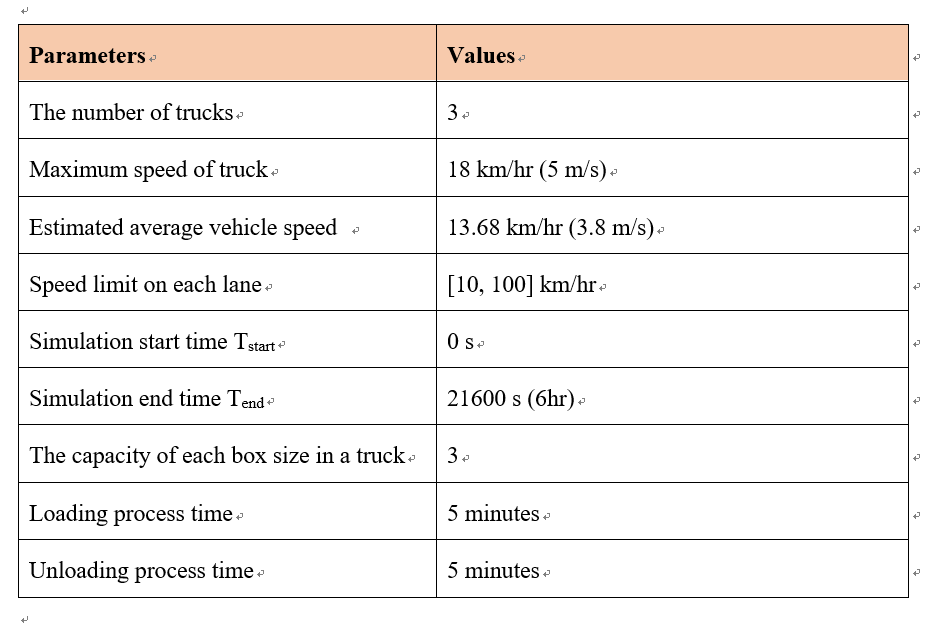
\includegraphics[width=1.0\textwidth]{./Thesis_figures/F7-4_parameters.PNG}
\caption{\large Parameters of simulation.}
\vspace{0.5cm}
\label{Fig:Parameters_of_Simulation}
\end{figure}

\subsection{Average Vehicle Speed Estimation}

As illustrated in Figure 7.5, the horizontal axis represents the different routes in Tainan downtown, and the vertical axis shows the vehicle's speed. Take the route 1 as an example, the route1 starts from Anping Fort to the Taiwan Tainan District Court, and the driving distance is 2.9 kilometers. In this case, the blue line represents the maximum speed of truck in SUMO, and the green line indicates the average vehicle speed in Google Map, and the orange line is real average vehicle speed in SUMO. Thus, according to the seven cases in this figure, to avoid the delay in delivery, the study sets estimated average vehicle speed to \textbf{"3.80"} m/s (13.68 km/hr).


\begin{figure}[H]
\centering
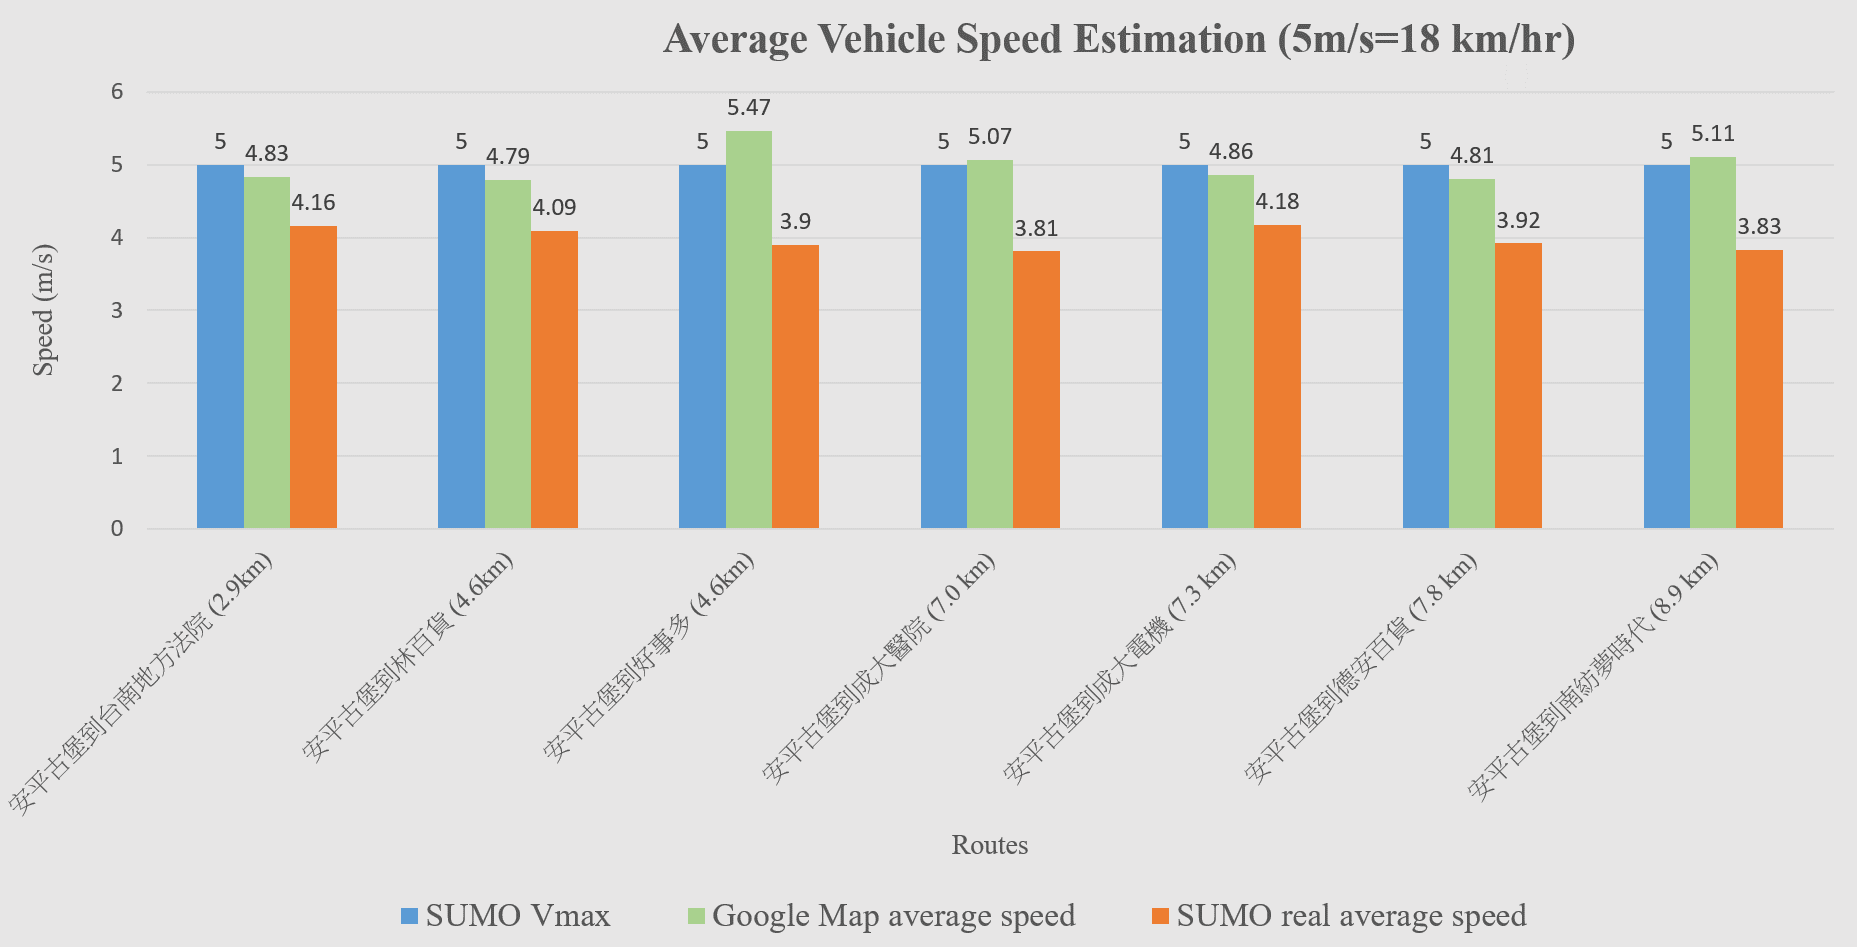
\includegraphics[width=1.14\textwidth]{./Thesis_figures/F7-5_speedEstimation.PNG}
\caption{\large Average vehicle speed estimation.}
\vspace{0.5cm}
\label{Fig:Average_vehicleSpeedEstimation}
\end{figure}

\section{Simulation Result}
It this section, there are five stages of simulation results, which includes simulation initialization, the sender’s request insertion, the loading process, the receiver’s request, and the unloading process.

As illustrated in Figure 7.6, the picture shows the simulation initialization without any request insertion. According to the time schedule in the left side of the Figure, each vehicle has different column color, which indicates the distinct routes. Take the vehicle 2 as an example, the system arranges blue route with one task in the right side of the Figure. Thus, the vehicle 2 would arrive to the Durban Department Store before 11:00 AM, and stay in the destination until 11:10 AM.

\begin{figure}[H]
\centering
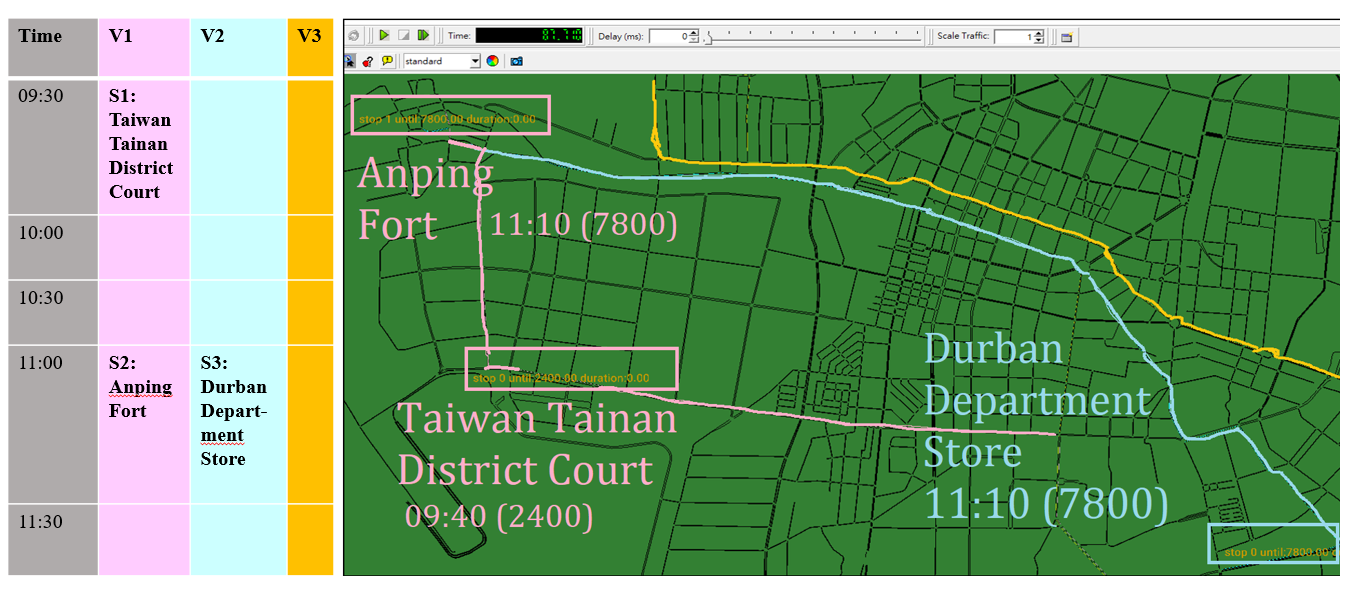
\includegraphics[width=1.12\textwidth]{./Thesis_figures/F7-6_initialization.PNG}
\caption{\large Initialization of Simulation.}
\vspace{0.5cm}
\label{Fig:Initialization_of_Simulation}
\end{figure}

As illustrated in Figure 7.7, the figure shows how the original route changes after receiving the sender’s request.
The left side of graph shows that when the simulation time is 1203 seconds, which means 09:20:03, and the user wants to pick 09:30 as the expected sender’s arrival time. Then, the vehicle 2 follows the yellow route. However, at the time of 1218 seconds, which means 09:20:18, the vehicle 2 replaces original blue route with yellow route and would stop at Hayashi Department Store until 09:40 AM.

\begin{figure}[H]
\centering
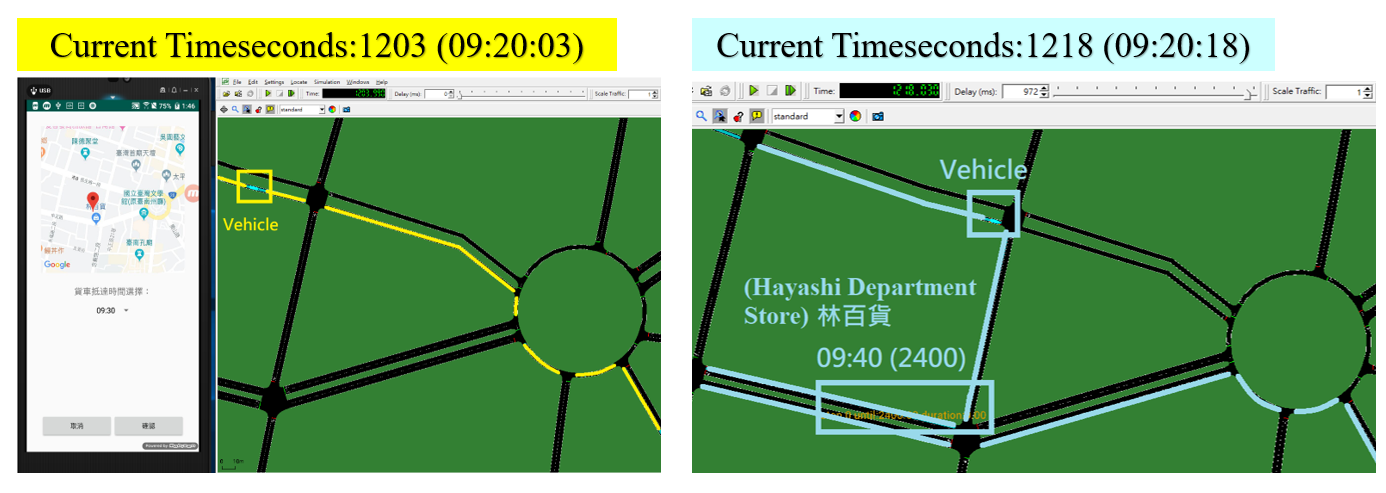
\includegraphics[width=1.12\textwidth]{./Thesis_figures/F7-7_senderRequest.PNG}
\caption{\large The Sender’s Request Insertion in simulation.}
\vspace{0.5cm}
\label{Fig:sender_request}
\end{figure}


As illustrated in Figure 7.8, the receiver’s phone in the left side of the figure gets the notification of finishing loading process at sender’s address in 09:35. The box index number “211” has the value of one, which means that the parcel exists in the vehicle 2. Thus, the receiver can start to select the expected arrival time of the parcel.

\begin{figure}[H]
\centering
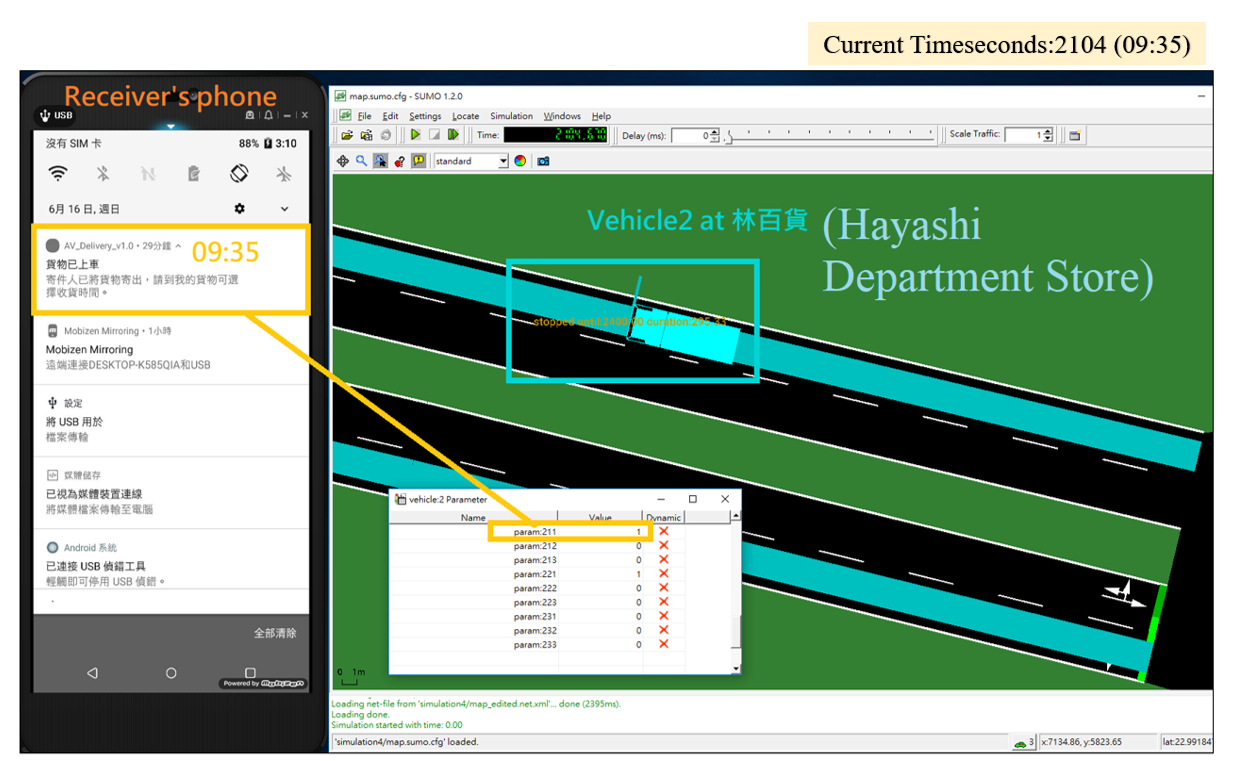
\includegraphics[width=1.12\textwidth]{./Thesis_figures/F7-8_loadingProcess.PNG}
\caption{\large The loading process at the sender’s sddress in simulation.}
\vspace{0.5cm}
\label{Fig:LoadingProcess}
\end{figure}


As illustrated in Figure 7.9, the left side of the figure shows that at the simulation time of 2104 seconds, which means 09:35:04, the receiver selects 10:00 AM as the arrival time. 
Moreover, at 09:36:16, the vehicle 2 replaces the original blue route with the yellow route after inserting the receiver’s request. This route in right side of the figure shows that the vehicle 2 would stop at the entrance of Kuang-Fu campus in National Cheng Kung University in 10:00.

\begin{figure}[H]
\centering
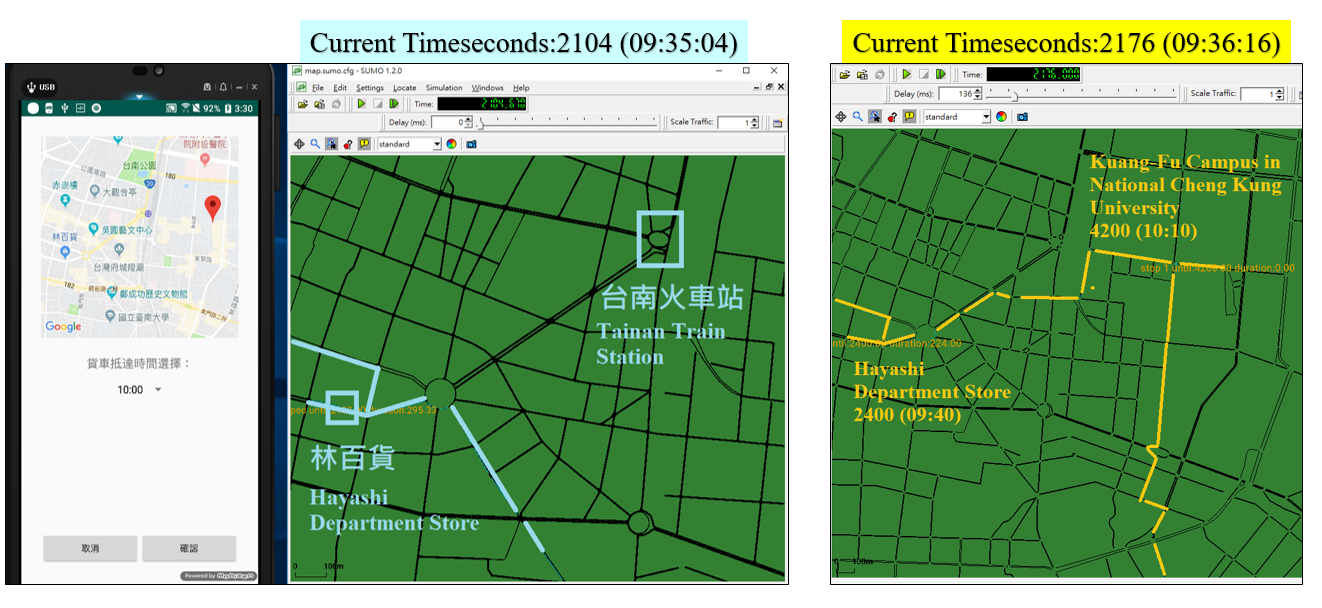
\includegraphics[width=1.12\textwidth]{./Thesis_figures/F7-9_receiverRequest.PNG}
\caption{\large The receiver’s request insertion in simulation.}
\vspace{0.5cm}

\label{Fig:Receiver_request}
\end{figure}

As illustrated in Figure 7.10, the receiver receives the arriving notification of the parcel at 10:00 AM. Then, at 10:07:29, the vehicle 2 finishes the unloading process and the parameters of box also changes. Besides, the vehicle 2 still has to stay in receiver’s address until 10:10 AM.

\begin{figure}[H]
\centering
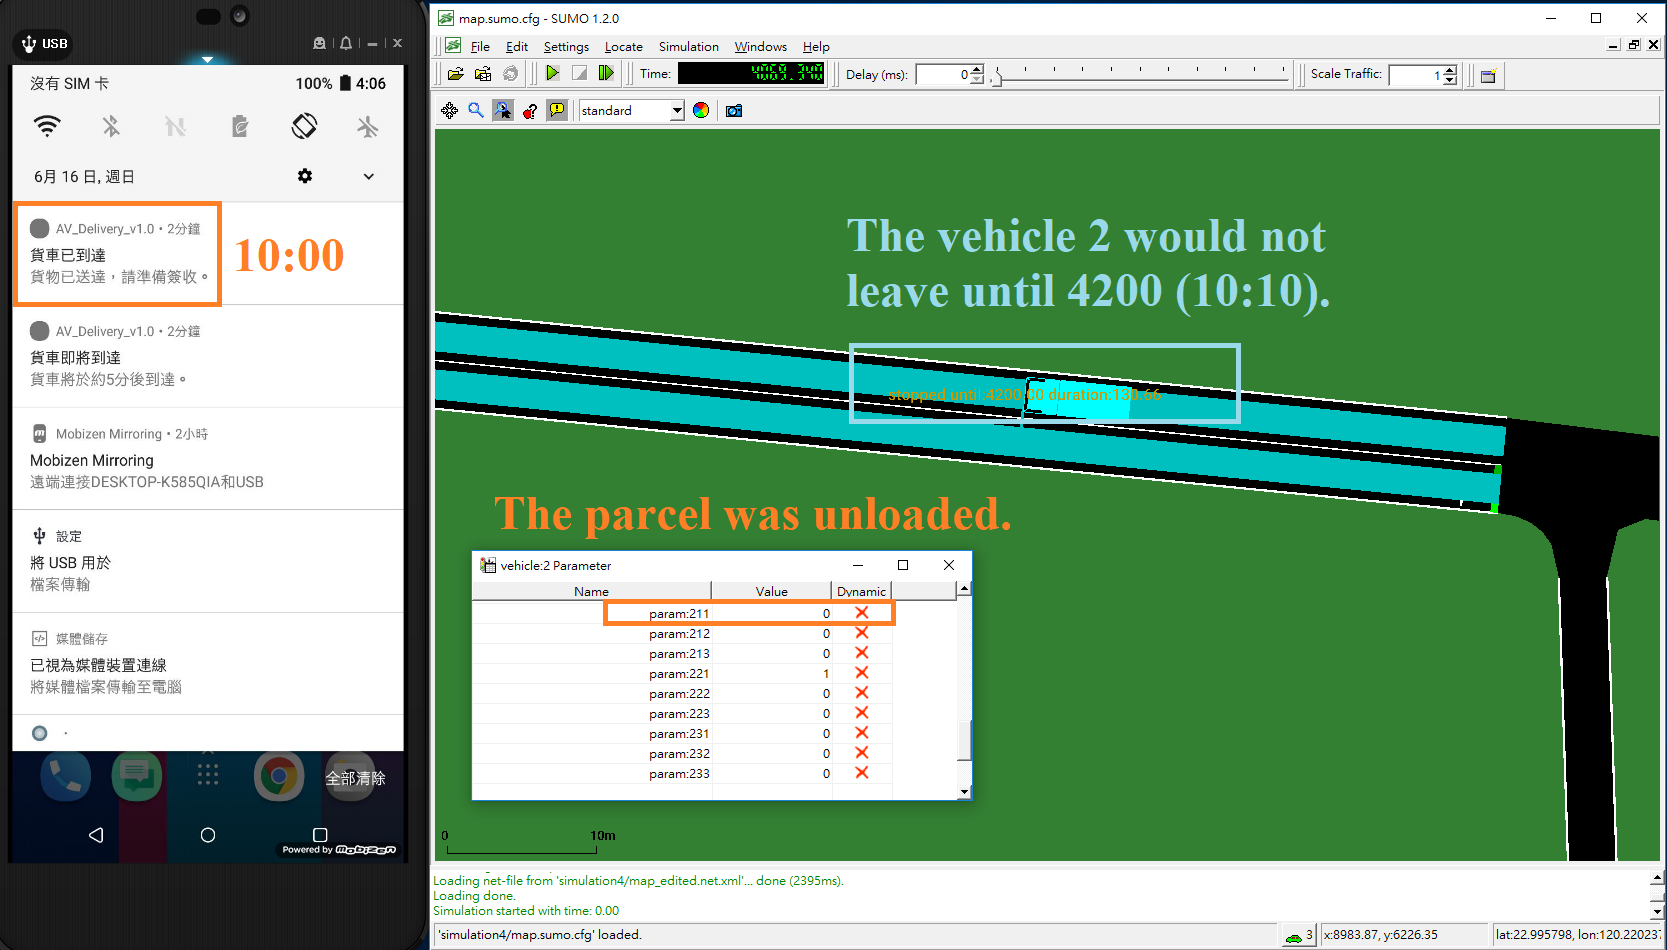
\includegraphics[width=1.12\textwidth]{./Thesis_figures/F7-10_unloadingProcess.PNG}
\caption{\large The unloading process at the receiver’s address in simulation.}
\vspace{0.5cm}
\label{Fig:unloading_request}
\end{figure}









%%%%%%%%%%%%%%%%%%%%%%%%%%%%%%%%%%%%%%%%%%%%%%%%%%%%%%%%%%%%%%%%%%%%%%%




\chapter{Conclusion and Future Work} \label{Chap:Conclusion}
%------------------------- Conclusion -------------------------%

\section{Conclusion}
In order to make the self-driving technology development companies have a platform to test and adjust the product before it is officially online, a system was designed and implemented to simulate the freight process of the self-driving delivery. This thesis handled the developing of a mobile application and the data transmission between apps and the simulation system. In terms of the mobile apps, an account system was accomplished to store user information, and the order functions were devised to send and display orders. For the purpose of performing the dispatching mechanism, SUMO server must be able to interact with mobile apps. Therefore, a socket server was built to receive and handle the data sent by apps. For similar reasons, FCM service was also be included in the system, and it can assist SUMO server in notifying users of mobile apps. As regards the database, a back-end server was built to supply the access interface of the database to the mobile apps. In contrast, SUMO server transfers data to the database directly because it is on the inner server side.


\section{Future Work}


} \end{thesis}

%------------------------- References -------------------------%
\singlespace {\large

\bibliography{Reference-Yen}

}

\bibliographystyle{IEEEtran}

\doublespace

\begin{vita}
%------------------------- Vita -------------------------%
\Thesisspace \large{

Kang Yen was born on December 3, 1993, in Yunlin, Taiwan.  He received the B.S. degree in Electrical Engineering from National Cheng Kung University, Taiwan, in 2017. In September 2017, he enrolled at the National Cheng Kung University as a master student in the Institute of Computer and Communication Engineering.

}\end{vita}

\end{document}

